% !TeX spellcheck = pl_PL
% --- Jest to instrukcją użytkownika, z której przeciętny użytkownik powinien się dowiedzieć wszystko,
% --- co jest mu potrzebne do jego prawidłowego użytkowania. Specyfikacja zewnętrzna dotyczy
% --- interfejsu użytkownika, sposobu uruchomienia i obsługi programu, formatu danych wejściowych i wyjściowych
\newpage
\part{\huge \textbf{Specyfikacja zewnętrzna}}
	\section{Uruchomienie gry}
		Gra nie wymaga instalacji. Wystarczy otworzyć plik \textit{Danmaku.exe} i gra uruchamiania się. Po włączeniu gry pojawia się ekran powitalny wraz z menu głównym.
		\begin{center}
			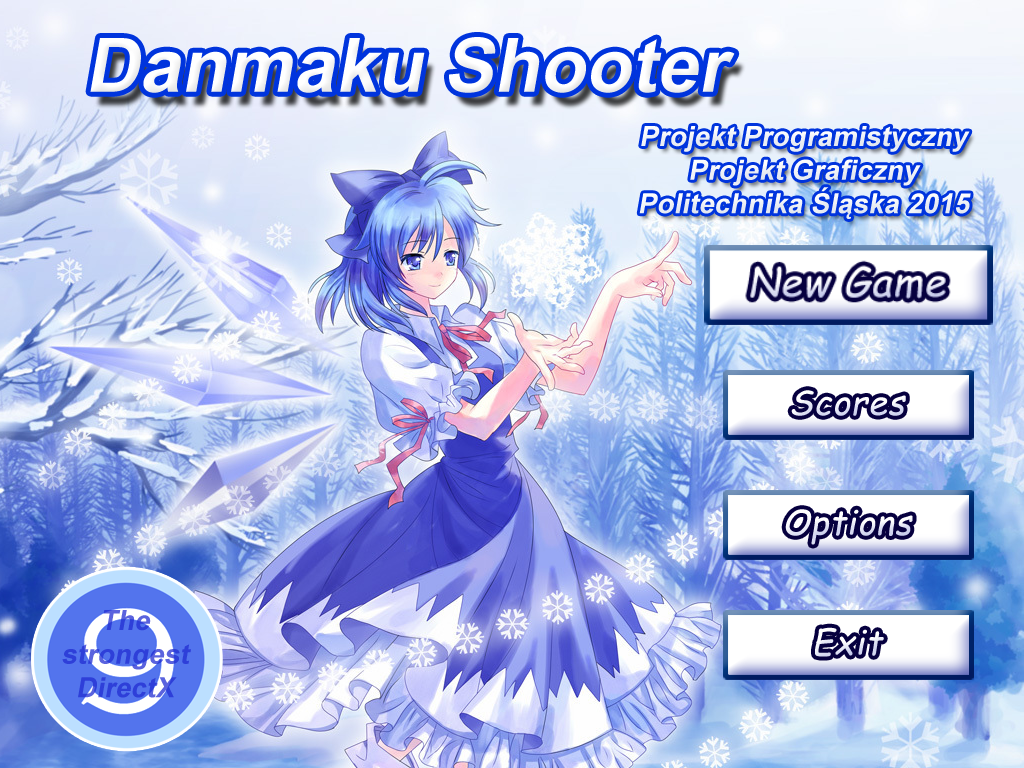
\includegraphics[width=0.7\textwidth]{./images/titlescreen_clear}
		\end{center}
		Użytkownik posiada 4 możliwości:
		\begin{itemize}
			\item Przycisk \emph{New Game} \tab - uruchomienie nowej gry
			\item Przycisk \emph{Scores} \tab - wyświetlenie wyników z poprzednich rozgrywek,
			\item Przycisk \emph{Options} \tab - konfiguracja gry
			\item Przycisk \emph{Exit} \tab - wyjście z aplikacji
		\end{itemize}
		Aktualnie wybrany przycisk pulsuje, co ułatwia wybór. Zatwierdzenia wyboru należy dokonać klikając przycisk ENTER.
	\newpage
	\section{Sterowanie}
		Domyślne sterowanie przez klawiaturę ustawione jest następująco:
		\begin{center}
			\begin{tabular}{|p{5cm}|p{5cm}|}
				\hline \textbf{Działanie} & \textbf{Klawisz(e)} \\ 
				\hline Przemieszczenie postaci & Strzałki: góra, dół, lewo, prawo \\ 
				\hline Strzelanie & Z \\
				\hline Wykorzystanie bomby & X \\
				\hline Tryb focus (spowolnienie) & Lewy Shift\\
				\hline Wyjście z gry & ESC\\
				\hline
			\end{tabular}
		\end{center}
		Klawisze sterujące można zmienić w menu \emph{Options} wedle uznania i wygody.
	\section{Konfiguracja}
		Po wybraniu przycisku \emph{Options} pojawia się menu konfiguracji.
		\begin{center}
			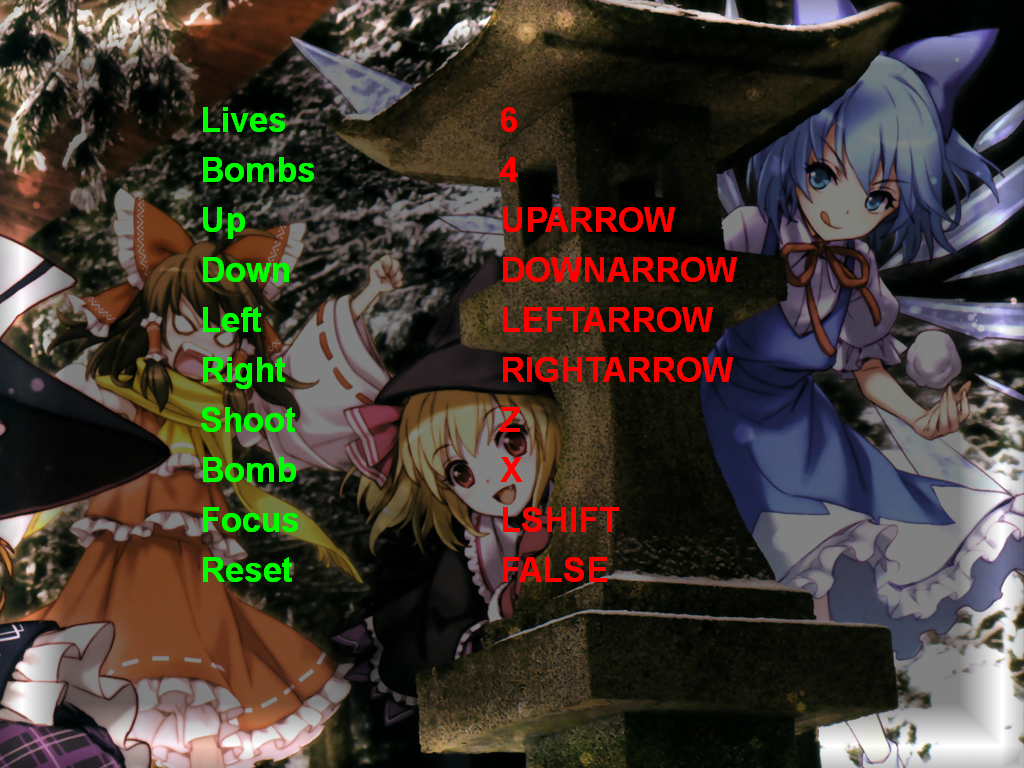
\includegraphics[width=0.7\textwidth]{./images/options_clear}
		\end{center}
		Użytkownik posiada możliwość zmiany:
		\begin{itemize}
			\item Początkowej liczby żyć, z którą rozpocznie nową grę. Aby zmienić tę wartość należy kliknąć\\ENTER, następnie strzałkami góra i dół zmienić liczbę (minimum 1, maksimum 8), i podaną wartość zatwierdzić ponownie klawiszem ENTER.
			\item Początkowej liczby bomb, z którą może rozpocząć grę. Obsługa zmiany tej liczby jest dokładnie taka sama jak dla żyć. 
			\item Klawisze sterowania. Klawiszem ENTER należy wybrać, który przycisk ma zostać zmieniony,\\a następnie potwierdzić wybór klikając wybrany przycisk na klawiaturze. Zmiana zostanie automatycznie zapisana.
			\item Przywrócenie ustawień domyślnych. Wybranie tej opcji powoduje zmianę ustawień klawiszy sterowanie na tę opisaną w podrozdziale Sterowanie, a także ustawia domyślną wartość liczby bomb\\i żyć. przywrócenie ustawień domyślnych należy zatwierdzić i można z tej decyzji się wycofać.
		\end{itemize}
		Należy pamiętać, że od startowej liczby żyć i bomb zależny jest ostateczny wynik punktowy nowej gry.
	\newpage
	\section{Tabela wyników}
		Po wybraniu przycisku \emph{Scores}, użytkownik ma możliwość podejrzenia, jakie wyniki zostały zapisane. Wyjścia z menu należy dokonać klawiszem ESC.
		\begin{center}
			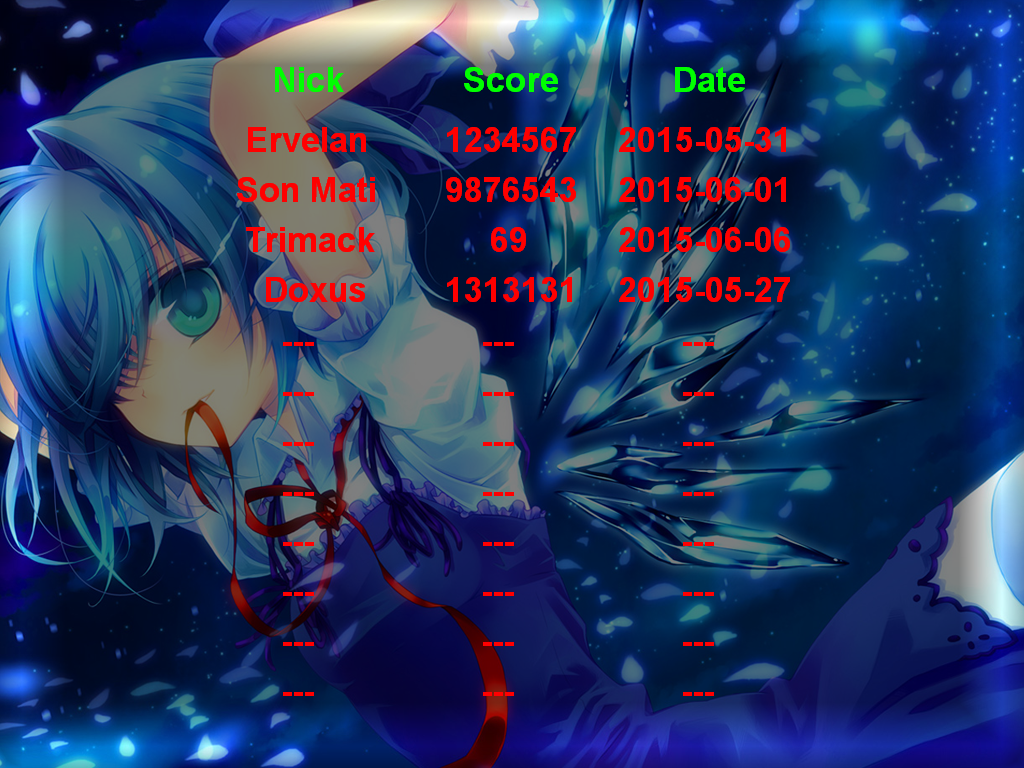
\includegraphics[width=0.7\textwidth]{./images/scores_clear}
		\end{center}
		Tabela z wynikami przedstawia rekordy z nickiem gracza, jego wynikiem punktowym oraz datą uzyskania i zapisania wyniku. Gra dopuszcza zapis tylko 12 wyników (nie muszą one być najlepszymi), w przypadku gdy gracz chce dodać swój wynik, a miejsca brakuje, musi nadpisać jeden z istniejących.
	\newpage
	\section{Gameplay}
		Po wybraniu przycisku \emph{New Game} rozpoczyna się nowa gra. Użytkownik rozpoczyna ją z zerową liczbą punktów i współczynnika \emph{graze}, oraz z najmniejszą mocą pocisków. Liczba żyć i bomb jest taka jak ustawione w Konfiguracji. Ekran gry prezentuje się następująco:
		\begin{center}
			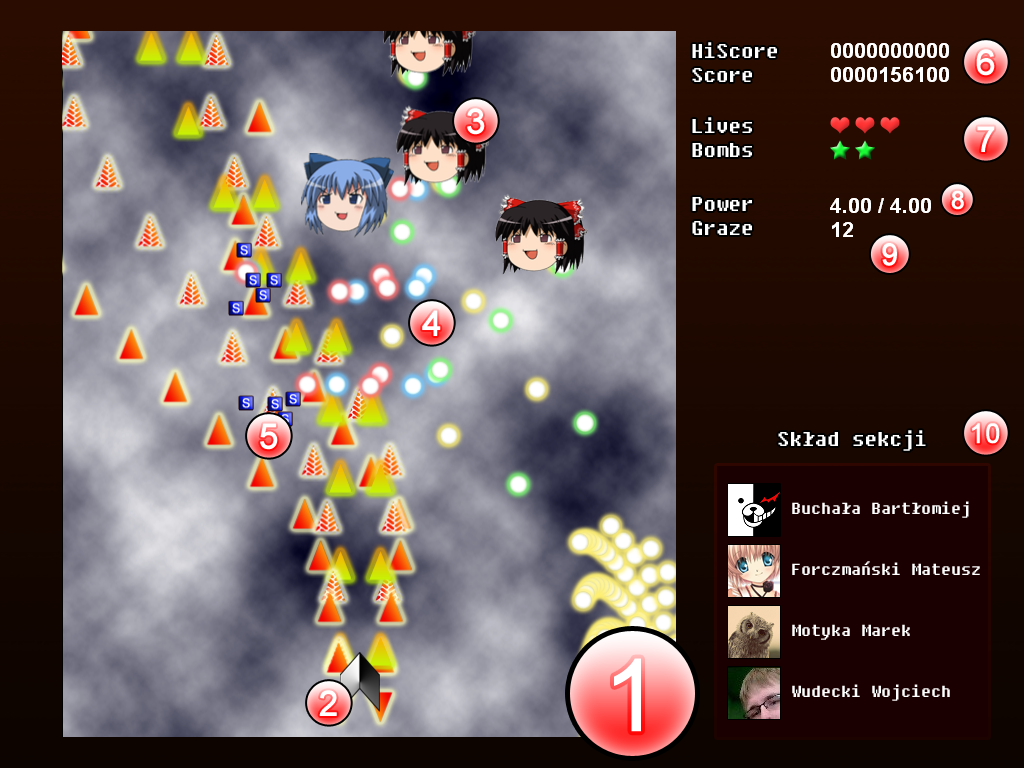
\includegraphics[width=0.7\textwidth]{./images/gameplay_clear}
		\end{center}
		\begin{enumerate}
			\item Plansza gry. Tutaj rozgrywa się cały gameplay: nie można wyjść poza jej granice, wrogowie pojawiają się zza boków i strzelają, a pociski za nimi znikają.
			\item Obiekt gracza, interaktywna część gry. Korzystając z klawiszy ruchu można nim poruszać. Jest źródłem pocisków i bomb.
			\item Wrogowie, do których należy strzelać i których należy unikać. Kontakt z nimi skutkuje stratą życia.
			\item Różnobarwne i różnokształtne wrogie pociski. Należy ich unikać, kontakt skutkuje stratą życia. Pociski mogą być wyeliminowane przez wykorzystanie bomby.
			\item Bonusy. Pojawiają się z niektórych wrogów, gdy zostaną oni pokonani. Zbieranie bonusów owocuje rożnymi efektami i wyróżniamy ich cztery rodzaje:
			\begin{itemize}
				\item Niebieski kwadrat z literą "S" \tab 
\includegraphics[width=10pt]{./images/bonusScore} \tab - dodatkowe punkty.
				\item Czerwony kwadrat z literą "P" \tab 
\includegraphics[width=10pt]{./images/bonusPower} \tab - dodatkowa moc
				\item Zielona gwiazda z literą "B" \tab 
\includegraphics[width=10pt]{./images/bonusBomb} \tab - dodatkowa bomba
				\item Czerwone serce z literą "L" \tab 
\includegraphics[width=10pt]{./images/bonusLife} \tab - dodatkowe życie
			\end{itemize}
			\item Wynik punktowy z aktualnej gry oraz porównanie go z aktualnym najlepszym wynikiem.
			\item Aktualna liczba bomb i żyć. Na początku gry jest taka, jak ustawiono w menu \emph{Options}.
			\item Aktualna moc. Można ją zwiększać zbierając odpowiedni typ bonusu. Strata życia skutkuje zmniejszeniem mocy. Zwiększanie mocy daje silniejsze pociski i zwiększa ich liczbę, co daje bardziej zaawansowany wzór.
			\item Liczba punktów \texttt{graze}. Licznik jest zwiększany, gdy gracz nie uderzy we wrogi pocisk, ale znajdzie się wystarczająco blisko, by móc powiedzieć, że się o niego "otarł". Graze zwiększa ostateczny wynik punktowy.
			\item Skład sekcji, który zrealizowała tę grę.
		\end{enumerate}
		
		
		
		
		
		